% !TEX root = ../paper.tex
\section{Experiment} \label{sec:experiment}
The four cross-device interaction techniques mentioned above were implemented and then evaluated in a lab study in order to judge their performance compared to each other. 
We are interested in knowing whether or not the different techniques with different target sizes have an effect on the efficiency, accuracy, and ease of use of pushing information to a large display. Therefore, we developed an application that would allow us to run experiments and test the effect of the different techniques and target sizes. 
We utilized a Microsoft Kinect, a 65' inch Panasonic television with a $1920 \times 1080$ resolution and a Samsung Galaxy SII to create the experimental application. 
An overview of the experiment setup can be seen in \Cref{fig:entireSetup}. 

\begin{figure}[H]
	\centering
	{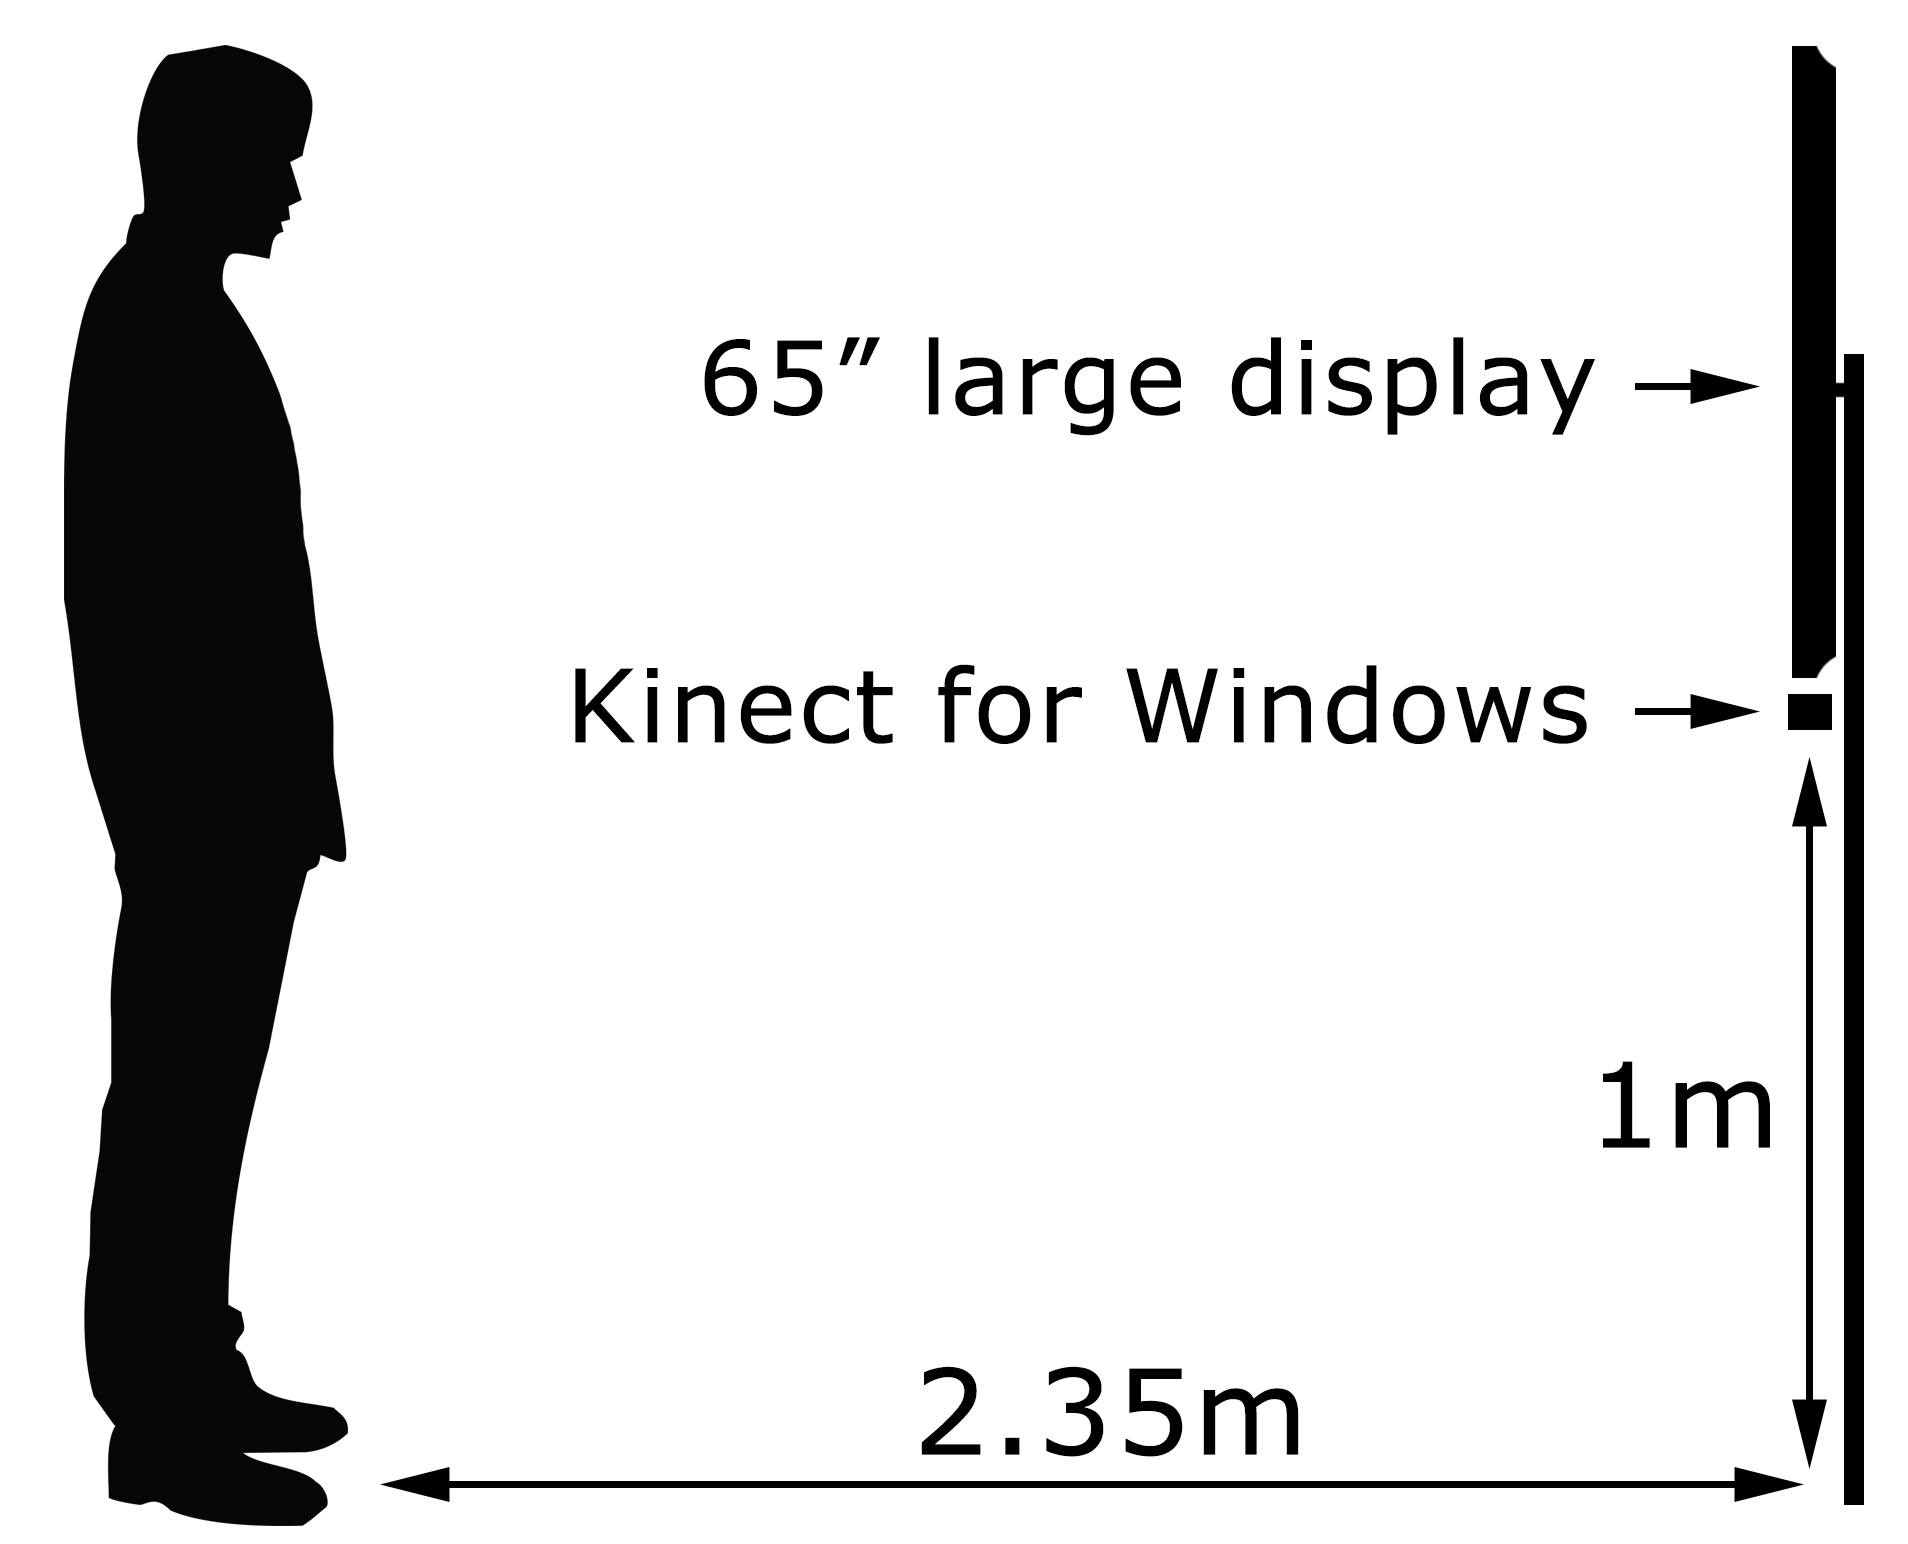
\includegraphics[width = 0.7\columnwidth]{images/SetupIllustration.jpg}}
	\caption{
		\protect An overview of the entire setup of our experiment.
	}
	\label{fig:entireSetup}
\end{figure}

\subsection{Implementation}

The 4 techniques (\swipe, \tilt, \throw, and \pinch) were implemented in order to push data onto the large display. 
They were implemented in a simple and short target practice application, where the goal was to "hit" the target on the display with the shown technique. 

A grid system was implemented in the test application, where each cell of the grid is a possible target. 
As mentioned, we were interested in measuring the effect of different target sizes on the different techniques, therefore the grid is implemented in two different sizes. 
The grid system can have large cells, where the grid is $5 \times 10$ cells and each cell is 61 pixels or 7.3 cm wide, or it could also have small cells, where the grid is $10 \times 20$ cells and each cell is 122 pixels, or 14.6 cm wide. 
The target is located in one of those cells, and scales accordingly to the size of the cell(See \Cref{fig:kinectScreen}).

The developed mobile application was simple. It showed two shapes, a circle and a square, which the user could choose to push to the display. The display would tell which shape was the correct one by having that shape as the target in one of the grid cells. We chose two shapes so that it did not become a search problem with users spending too much time searching for the correct shape. We wanted the user to spend some time orienting him or her self with the phone and not just simply performing the gesture without paying any attention to the phone at all. The phone screen can be seen in \Cref{fig:phoneScreen}.

Users would control the pointer on the large display with their hands. 
Which ever hand was closest to the screen would determine the position of the pointer on the large screen. 
This meant that users could switch hands whenever they pleased at any point during the test. 

The \pinch technique was implemented with the help of the Kinect and the touch screen on the mobile phone. 
This technique started by having the user pinch the shape on the screen of the mobile phone and close his or her hand around it, as if to grab it. 
The Kinect would then look for a opening of the hand motion, on the pointer hand, and take that as the target point.

The \swipe technique was implemented with the touch screen of the phone. 
Here, we detected when a significant swipe happened on the screen, and then use the pointer location to place the shape that was swiped up onto the screen. 

The \throw technique was also implemented with the help of the Kinect and the accelerometer on the mobile phone. 
The Kinect looked at the user to recognize when a user moved the mobile phone from 10 centimeters behind the hip to 10 centimeters in front of the hip. 
At the same time, the phone detects when a significant change in the accelerometer happened, so to not simply detect an unintentional wave of the arm. 
The Kinect would then use the position of the other hand to see where on the screen the user intended to perform the \throw technique towards. 

The \tilt technique was implemented mostly with the accelerometer of the phone, by checking for a significant change in the z and y axis of the accelerometer, as if tilting the phone forward. 

\begin{figure}[H]
	\centering
	\subfloat[]{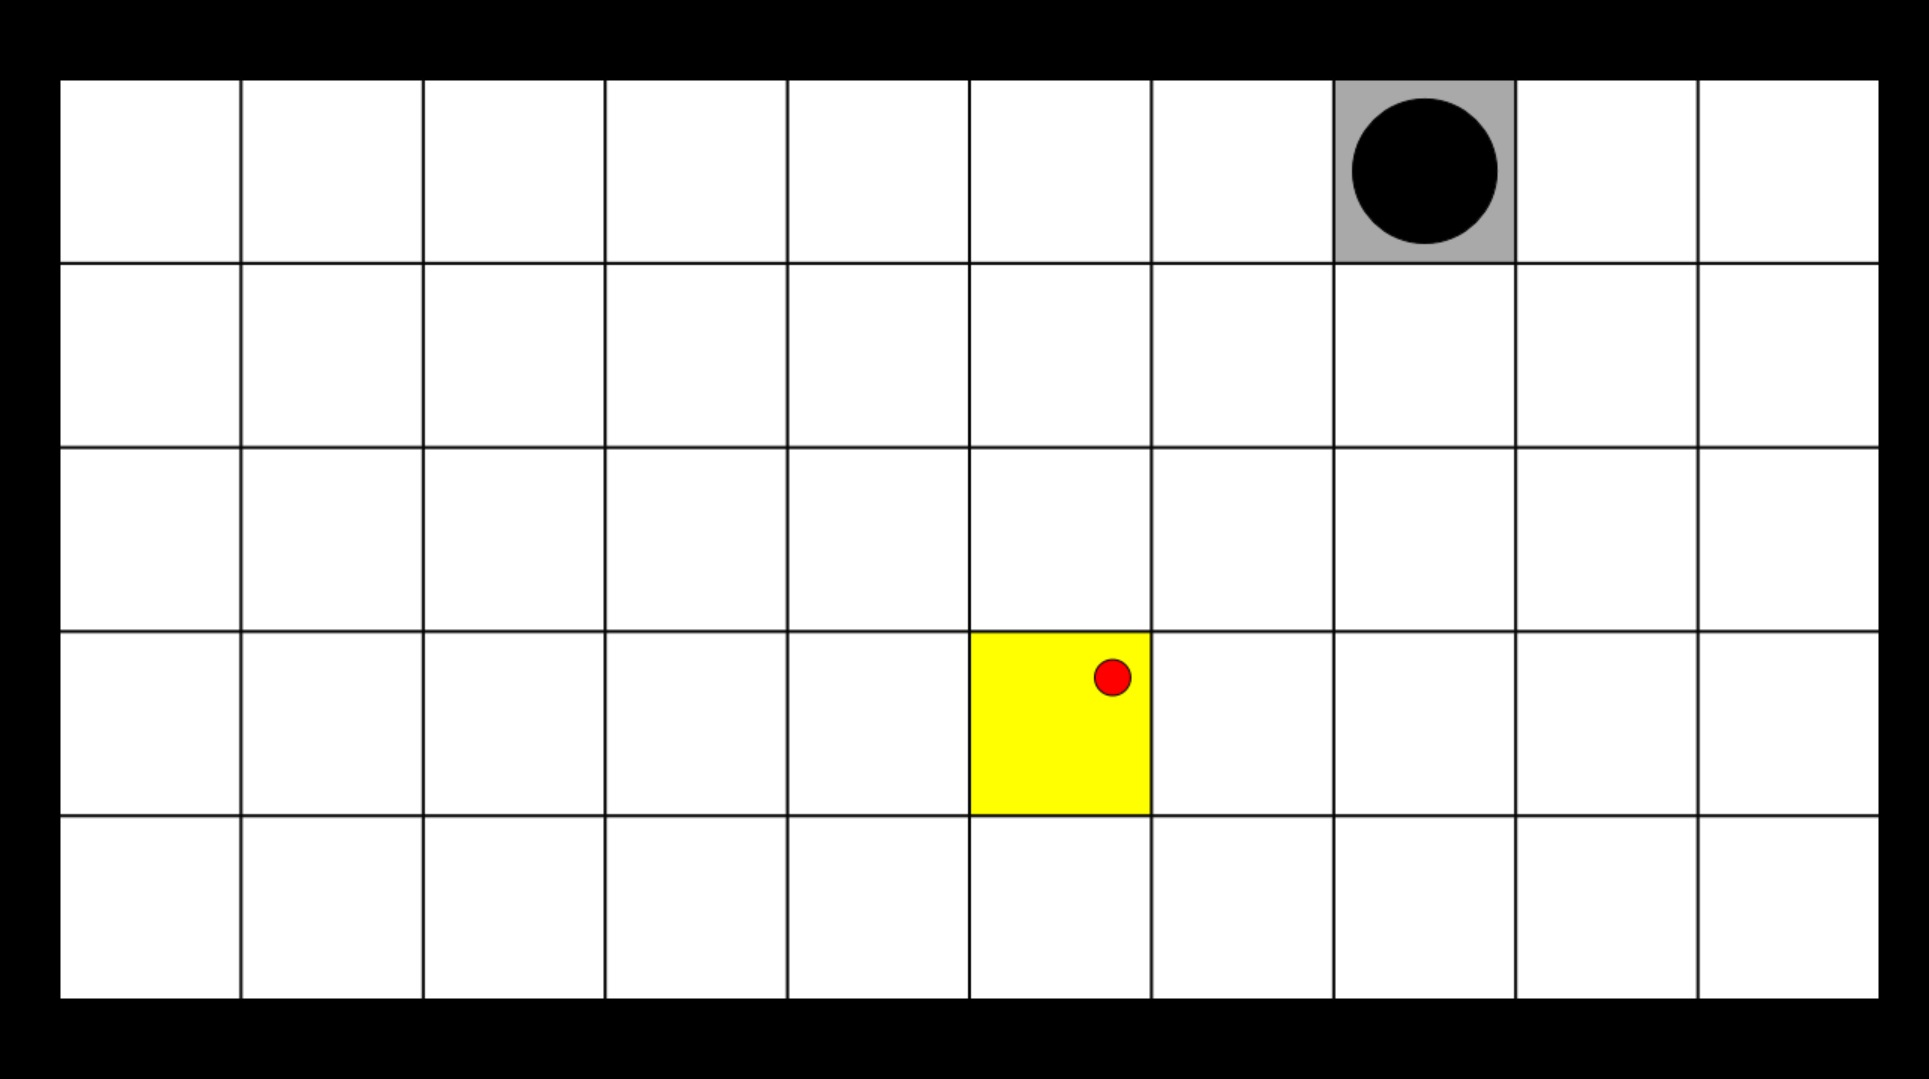
\includegraphics[width = 0.69\columnwidth , height = 3.3cm ]{images/kinectScreen.jpg}\label{fig:kinectScreen}} 
	\qquad
	\subfloat[]{
\includegraphics[height = 3.3cm ]{images/phoneScreenshot.png}\label{fig:phoneScreen}}
	\caption{
		\protect\subref{fig:kinectScreen} The large display screen of the application, with the red dot in the highlighted square as the starting point and the black circle as the target.
		\protect\subref{fig:phoneScreen} The phone screen showing the two shapes.
	}
	\label{fig:allSetup}
\end{figure} 

\subsection{Experimental Design}\label{sec:expdesign}
The experiment was conducted as a within-subject research, with the four different interaction techniques and two target sizes as independent variables. 

The within-subject research was chosen because we wanted to minimize the amount of subjects needed in order to get a significant result. We also believed that the learning effect would not be as pronounced since the four techniques are very different from each other. 
We chose to investigate techniques because we were interested in learning about the way people interact with large displays, and the two target sizes to investigate precision. Sometimes users need to be as precise as possible, and sometimes they just need to be able to interact with a large display. 

For the dependent variables, different measures of completion time and hit success were used, as well as a short questionnaire to get the user's satisfaction with regard to the given interaction technique. 
Which technique started the test was randomized in order to mitigate the learning effect on the entire set of tests. 
In the end, the \pinch gesture started 26.4\% of all tests, \swipe started 22.7\% of all tests, \throw started 24.5\% of all tests, and \tilt started 26.4\% of all tests. 
All of this was automatically logged, and every test session was also video recorded in order to be able to go through them in case we wanted to go into detail in one of the test sessions.

A simple logging mechanism was developed, which created a unique file for each user and outputted all attempts into that file. 
In the end, the result was a list of 53 files, one for each test participant, where each file would have a list of attempts and target size switches. 
Each attempt would have a time stamp, whether the user hit the target or not, whether he selected the correct shape, were the target was, and where the participant hit. 
These where the following measures that we were able to deduce from the log files that were generated: 

\textit{Total Time:} This was the time each user spent completing the test for a given interaction technique. 
This was measured from the time each user had hit his first target after a practice period of three tries until he had hit his last target. 
There were a total of 18 targets, plus the first target used for calibration. 

\textit{Time per target:} This was the time each user spent hitting each of the targets. 
This was measured as the time since each user last hit a target until he hit the next one.

\textit{Hit success:} Whether or not each user hit the given target. 
Current pointer and target position (in both cell and pixels coordinates) were also recorded in order to give a precise measure of accuracy for each attempt in terms of \textit{distance to target}. 

\textit{Ease of use:} Each user was given a questionnaire after having gone through each interaction technique. 
There were 6 questions, all taken from the USE questionnaire \cite{lund2001measuring}. 
These were asked to get an understanding of how useful and easy to use each technique was. 
The 6 questions were the following: 

\begin{itemize}
	\item It is easy to use
	\item Using it is effortless
	\item It is easy to learn to use
	\item I can use it successfully every time
	\item I quickly became skillful with it
	\item I learned how to use it quickly
\end{itemize}

Users were able to rate their answers to each question on a 7 point Likert scale. 
We also wrote down any comments made during the experiment and combined them with the questionnaire responses to get a better understanding of the user's response to each of the techniques. 

\subsection{Participants}
In total, 53 people took part in our experiment, which was conducted in a usability lab. 
The participants where between 20-45 years old (M: 24.4, SD: 4.3) and were between 1.63 and 1.95 meters tall (M: 1.82, SD:7.8). 
88.7\% of users were right handed, 90.6\% were male, and 96.2\% of them were smartphone users. 
Of those who owned smartphones, they had owned one for 2-15 years (M:5, SD:2.1). 
They were recruited through a mixture of our social network and recruitment posters around the campus. 

\subsection{The Experiment}

Each test subject was taken into the usability lab and given a short introduction to what we were doing and why. 
We then explained how the system worked and what they had to do. 
We would hand them a phone, ask them to stand on a marked cross, so that the distance to the screen would always be the same, and start the test.

The application chose at random one of the four techniques and displayed a short explanatory movie of how to perform the technique on a screen right beside the main application display(See \Cref{fig:tutVideo}).

\begin{figure}[H]
	\centering
	\subfloat[]{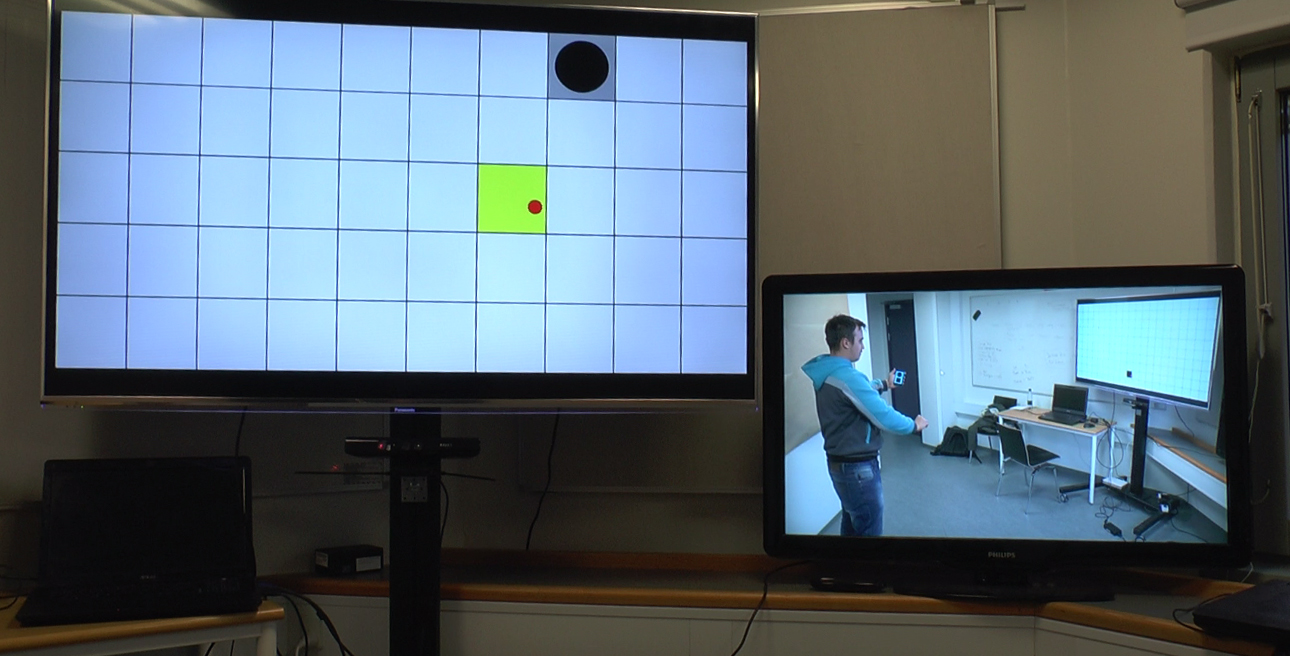
\includegraphics[width = 0.49\columnwidth]{images/setup.jpg}\label{fig:tutVideo}}
	\hspace{0.01\columnwidth}
	\subfloat[]{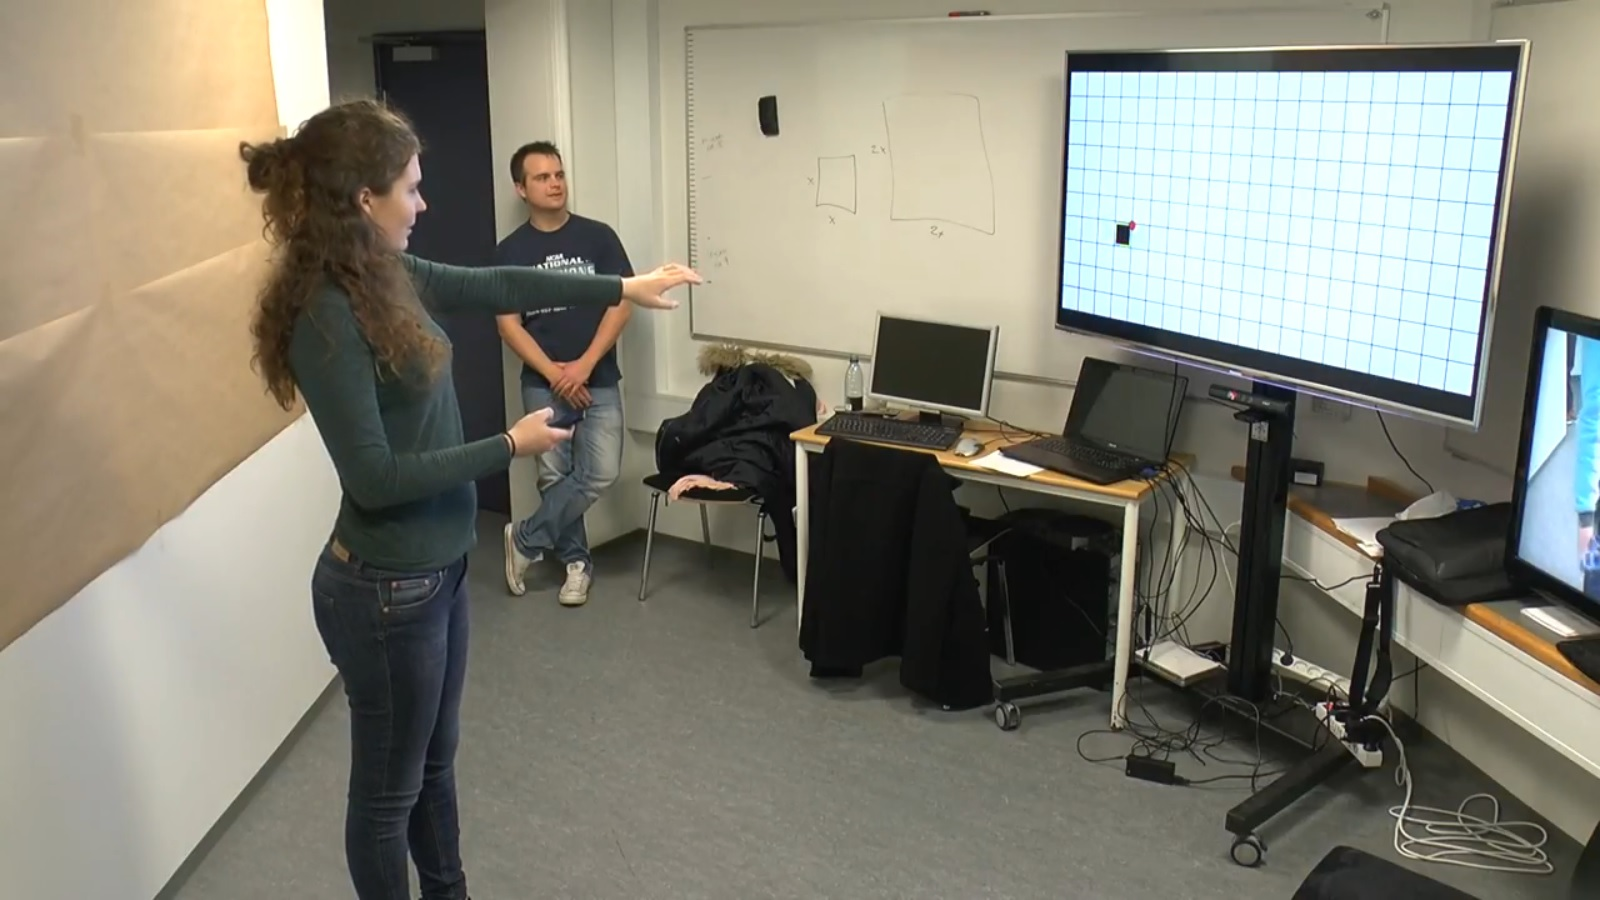
\includegraphics[width = 0.49\columnwidth]{images/experiment.jpg}\label{fig:experiment}}
	\caption{
		\protect\subref{fig:tutVideo} The main screen on the left with the tutorial video screen on the right.
		\protect\subref{fig:experiment} The experiment in progress, as seen from the right. 
	}
	\label{fig:setup}
\end{figure} 

The user would then have three practice attempts, in order to get familiar with the technique. 
Nothing was logged during the practice phase.
A shape would appear, either a square or a circle, at one of the cells in the grid. 
The user would have to choose the correct shape on the phone and perform the technique with that shape selected. 
The shapes on the phone (\cref{fig:phoneScreen}) would randomly change positions, so that the user would have to check the phone after every technique. 
The target would also randomly change size from small to large or vice-versa. 
In reality, the target sequences where hard coded by us in such a way that there was an equal distribution of small and large targets. 
We also made sure that there was an equal distribution of distances between each target. We classified them as short jumps, medium jumps, and long jumps. 
A short jump was 2 large cells(4 small cells), a medium jump was 4 large cells(8 small cells), and a large jump was 6 large cells(12 small cells).  
After a practice phase of 3 practice targets, a calibration start target would be shown. This is so that we could calculate the distance between all other targets correctly. 
The user would then go through the rest of the test (18 targets), going through a total of 22 targets. 

That means that our experiment had the following list of conditions:
\begin{itemize}
	 \item Technique (4)
	 \item Target size (2)
	 \item Target jump distance (3)
	 \item Repetition (3)
\end{itemize}

This means that each user had a total of $4 \times 2 \times 3 \times 3 = 72 $ targets.

After going through every target for one technique, the user would then be asked to fill in the short questionnaire regarding the technique just tried in terms of how natural it felt based on ease of use measures. 

This entire process would be repeated four times in total, once for each technique. 
After that, we presented them with a short demographics questionnaire, in order to better understand the user. 
We asked them about their age, height, if they were left or right handed, if they had a smartphone, for how long, if they had any experience with a Kinect, Wii, Playstation Move, or any other similar air gesture based technologies, and how often they used them. 
Finally, we thanked them for their time.
The entire test took on average 15 minutes. 